\begin{abstract}
Agentic RAG often persists retrieved text as long-term memory, allowing stale, contradictory, unsupported, or malicious writes to influence later sessions. ClaimLedger is an append-only, claim-level integrity layer: it decomposes writes into atomic claims and records provenance, valid and transaction time, trust tier, confidence, lifecycle state, supersession, and conflict relations. Status-aware temporal, conflict, provenance, and quarantine gates produce an auditable retrieval decision. A SQLite prototype runs the official REALTALK release (10 human-human conversations, 219 sessions, 8,944 turns, 726 evidence-linked annotated memory questions) with controlled conflict/poison overlays and 209 timestamp-derived transitions: 2,387 mechanism cases. Removing the conflict gate drops exact active-claim accuracy from 1.000 to 0.696, removing valid-time filtering drops temporal accuracy to 0.000, and naive active memory reaches only 0.392 exact accuracy with 1.000 poison activation; a lexical-retrieval control given the same gold labels but no gate reproduces the naive failure, confirming the deltas come from the ledger gates, not the labels. Under oracle labels (relations supplied, not extracted), the gates execute perfectly across three deterministic seeds---gate-correctness checks given gold labels, not evidence of autonomous label production, end-to-end QA superiority, or adaptive-attack resistance.
\end{abstract}

\begin{IEEEkeywords}
agent memory, retrieval-augmented generation, provenance, temporal validity, memory poisoning, trustworthy AI agents
\end{IEEEkeywords}

\section{Introduction}\label{sec:intro}

\IEEEPARstart{R}{etrieval}-augmented generation (RAG) grounds language-model outputs in external memory~\cite{lewis2020rag}; agentic RAG adds planning, tool use, retrieval control, and multi-step reasoning~\cite{singh2025agenticrag}. Long-term memory persists observations, preferences, task outcomes, and inferred knowledge across sessions~\cite{hu2025memorysurvey}, turning one-session errors into durable state.

Even without security concerns, long-term memory remains difficult: LoCoMo and REALTALK test multi-session recall, while LongMemEval adds extraction, temporal reasoning, updates, and abstention \cite{maharana2024locomo,realtalk2025,wu2024longmemeval}. Graph and hierarchical systems improve retrieval and personalization but usually optimize response quality rather than the integrity of an agent's beliefs \cite{rasmussen2025zep,kang2025memoryos,xu2025amem}.

The security problem is concrete: AgentPoison demonstrates backdoors from poisoned memory without fine-tuning; MINJA injects malicious records through query-only interaction; Sleeper memory poisoning studies delayed fabricated memories; and MPBench systematizes exploitable write channels \cite{chen2024agentpoison,dong2025minja,pulipaka2026sleeper,dash2026mpbench}.

Related methods address parts of the problem: MRAG\slash TempRAGEval and ChronoQA investigate time-sensitive evidence; T-GRAG models evolving knowledge; MIRAGE exposes citation-attribution failures; TierMem links summaries to raw logs; and Mneme proposes a bitemporal contradiction ledger~\cite{zhang2024mrag,chen2025chronoqa,li2025tgrag,qi2024mirage,zhu2026tiermem,mneme2026}. The open question is whether one memory layer can preserve claim integrity under temporal change, source conflict, and adversarial writes.

ClaimLedger exposes individual-claim status before generation. It stores append-only transactions with provenance, valid and transaction time, confidence, trust tier, lifecycle state, supersession, and conflict relations. Unlike methods that address only temporal retrieval or contradiction resolution, it integrates temporal validity, conflict disclosure, and poisoning quarantine while complementing vector, graph, and temporal retrieval.

The research question for this prototype paper is:

\begin{quote}
Can a claim-level memory integrity layer reduce invalid active-memory states caused by stale claims, unresolved conflicts, and poisoned writes in long-term agentic RAG?
\end{quote}

The contributions are a claim-level bitemporal schema and lifecycle model, an executable prototype with deterministic perturbation runners and ablations, mechanism-level evidence from authentic REALTALK dialogue evidence and timestamps, and the empirical finding that downstream abstention behavior over the ledger packet is a joint model-and-strategy property rather than a ledger effect that deployments must calibrate. The experiments measure admissible active claims, not downstream free-form answer quality.

\section{Related Work}\label{sec:related-work}

\subsection{Long-Term Agent Memory}\label{sec:related-agent-memory}

Recent surveys distinguish agent memory by form, function, and dynamics, including factual, experiential, and working memory \cite{hu2025memorysurvey}. LoCoMo, REALTALK, and LongMemEval expose failures in cross-session recall, temporal reasoning, updating, and abstention \cite{maharana2024locomo,realtalk2025,wu2024longmemeval}. Zep, MemoryOS, A-MEM, Mem0, and reflective memory management improve persistent-memory storage, updating, retrieval, and generation \cite{rasmussen2025zep,kang2025memoryos,xu2025amem,mem02025,rmm2025}. Mneme adds claim-level storage through a Postgres bitemporal contradiction ledger for token-frugal reasoning \cite{mneme2026}. Several of these systems expose graph or hierarchical structure for richer retrieval. ClaimLedger is complementary to graph memory rather than a replacement: a graph can still supply candidate claims, while the ledger governs their admissibility by lifecycle status, valid time, conflict state, and trust tier before retrieval. The contribution is the governance gate, not the retrieval structure.

These systems generally optimize downstream response quality. Mneme emphasizes token efficiency and collective reconciliation; ClaimLedger treats memory as commitments whose eligibility is governed before retrieval. Candidate, quarantined, active, and superseded states support auditable trust-tiering when sources disagree or facts change. The specific axis ClaimLedger adds over Mneme-style bitemporal claim storage is twofold: poisoned-write quarantine is a first-class lifecycle state rather than a retrieval-side filter, and admissibility is decided as a generation-time gate before retrieval rather than as a post-retrieval ranking signal.

\subsection{Temporal RAG and Stale Knowledge}\label{sec:related-temporal-rag}

Temporal RAG aligns retrieved evidence with query time. MRAG introduces TempRAGEval and shows that off-the-shelf retrievers struggle with temporal perturbations \cite{zhang2024mrag}; ChronoQA benchmarks temporal QA over news \cite{chen2025chronoqa}; and T-GRAG encodes evolving knowledge in temporal graphs and retrieval stages \cite{li2025tgrag}. These methods are relevant because stale memory is a temporal-validity failure.

ClaimLedger targets lifecycle management rather than ranking alone: valid-time metadata determines eligibility, while lifecycle states distinguish active, expired, superseded, conflicted, quarantined, and rejected records.

\subsection{Source Attribution and Provenance}\label{sec:related-provenance}

RAG citations do not guarantee faithful source use. MIRAGE shows that self-citing LLMs may refer to non-existent or unsupported sources \cite{qi2024mirage}, and citation-faithfulness work shows that a correct answer may still cite the wrong evidence \cite{wallat2025correctness}. TierMem is especially close because it links summary memories to raw logs and escalates when summaries are insufficient \cite{zhu2026tiermem}.

ClaimLedger moves governance from summaries to atomic claims and adds temporal scope, transaction history, confidence, conflict sets, and explicit poisoning-quarantine states.

\subsection{Memory Poisoning}\label{sec:related-poisoning}

Persistent memory is an attack surface. AgentPoison demonstrates backdoor poisoning against RAG-agent memory and knowledge bases \cite{chen2024agentpoison}; MINJA injects records through interaction without direct store access \cite{dong2025minja}; Sleeper memory poisoning studies delayed attacks in stateful assistants \cite{pulipaka2026sleeper}; and MPBench systematizes memory write channels, structural vulnerabilities, and attack classes \cite{dash2026mpbench}.

ClaimLedger is not a complete security solution. Its narrower claim is that provenance binding, write quarantine, trust tiering, temporal validity, and conflict-aware retrieval can reduce activation of untrusted inputs.

\subsection{Knowledge Representation, Provenance, and Temporal Data}\label{sec:related-knowledge-rep}

ClaimLedger draws on truth-maintenance and belief-revision systems \cite{doyle1979tms,dekleer1986atms,agm1985belief}, database provenance \cite{green2007provenance,cheney2009provenance}, and the valid-time/transaction-time distinction \cite{snodgrass1995temporal}. A claim may remain historically true without remaining eligible. ClaimLedger is compatible with graph-memory extraction, storage, retrieval, and evolution, but adds explicit generation-time admissibility rules \cite{yang2026graphmemory}.

\section{Problem Formulation}\label{sec:problem-formulation}

Let an agent memory store receive observations $O = \{o_1,\ldots,o_n\}$ from user interactions, tools, documents, webpages, and prior actions. A conventional system maps them to retrievable units $m_i$ (chunks, summaries, or graph nodes); a query $q$ retrieves $R(q)$ for answer or action generation.

ClaimLedger inserts a claim layer between observation and retrieval. Each observation may produce zero or more atomic claims:

\[
\boldsymbol{c = \langle s,p,o,E,v_f,v_u,tx_f,tx_u,\tau,\gamma,\sigma \rangle}
\]

Here $s,p,o$ are subject, predicate, and object; $E$ is the evidence pointer; $v_f,v_u$ are valid-from/until times; $tx_f,tx_u$ are the interval during which the ledger accepted the record; $\tau$ is trust tier; $\gamma$ is confidence; and $\sigma$ is lifecycle status. The interval is append-only: correction, rejection, or supersession creates a new transaction rather than overwriting history.

The system answers three governance questions:

\begin{enumerate}
\item \textbf{Write eligibility:} Should an extracted claim become active memory, remain quarantined, or be rejected?
\item \textbf{Temporal eligibility:} Is the claim valid for the query time or superseded by a newer claim?
\item \textbf{Conflict eligibility:} Is the claim contradicted by another claim with stronger or more recent evidence?
\end{enumerate}

\subsection{Definitions and Invariants}\label{sec:definitions-invariants}

The bitemporal model records two time axes per claim: \textit{transaction time} (when the fact was written into the ledger) and \textit{valid time} (when the fact holds in the world). The gates preserve the following invariants: (I1) append-only history---no transaction overwrites a prior state; (I2) valid-time ordering---a claim inactive at query valid time is never returned as active; (I3) conflict disclosure---a claim with an unresolved contradicting relation is flagged rather than silently returned; (I4) quarantine---a claim whose provenance or trust tier fails the policy is withheld from retrieval. These invariants are the contract the mechanism evaluation checks; the ablations test what fails when one is removed.

\textbf{Claim.} An atomic proposition extracted from an observation and linked to evidence; extraction does not imply truth.

\textbf{Evidence.} An immutable pointer to a raw span, document, session, tool trace, or external source from which a claim was derived.

\textbf{Valid time.} The interval for which the claim is asserted to hold in the modeled world.

\textbf{Transaction time.} The interval for which the ledger accepted a claim record as memory state.

\textbf{Active belief.} A claim currently eligible to influence generation; it must have admissible provenance and temporal eligibility and no unresolved higher-priority conflict.

\textbf{Conflict.} Two claims that cannot both hold for the same subject and predicate over overlapping valid time under the current ontology or task-specific contradiction rules.

ClaimLedger enforces three invariants: every active claim points to evidence; every state transition is a new ledger transaction; and retrieval exposes conflict or uncertainty rather than collapsing incompatible claims into one unqualified answer.

\subsection{Eligibility Semantics and Worked Trace}\label{sec:semantics-trace}

For query time $t$, let $V(c,t)$ mean $c.v_f\le t<c.v_u$, treating a missing lower or upper bound as open. Formally, $A(t)=\mathrm{filter}(L,\,\sigma=\mathrm{active},\,V(c,t),\,E(c)\ne\mathrm{null})$, where $E(c)$ is the immutable evidence reference. Conflicted and quarantined records are retained for audit but excluded from $A(t)$; a conflicted record is disclosed in $C(t)$, and a quarantined record is disclosed in $Q(t)$. A supersession edge is valid only when the two claims share the governed $(s,p)$ key and the newer claim's valid interval replaces the older interval. In the headline prototype, conflict and supersession edges are supplied by the controlled case adapter; extraction and automatic relation discovery are evaluated separately.

Worked trace: an observed claim $c_1=(s,p,o_1)$ with evidence $E_1$ and valid time $t_q$ is appended active; an incompatible $c_2=(s,p,o_2)$ with overlapping validity appends contradiction edges, marks both conflicted, and discloses the pair; an untrusted $c_3$ is appended quarantined. The retrieval packet therefore contains eligible claims plus conflict/quarantine notes, while preserving all three records for audit.

Audit example: to reconstruct why $c_1$ was returned as active at query time $t_q$, an auditor reads the append-only transaction log for $c_1$: its single write event at transaction time $tx_f$, its evidence pointer $E_1$ (an immutable span in the raw session), its valid-time interval $[v_f,v_u)$ containing $t_q$, its trust tier and confidence above the activation threshold, and the absence of any supersession or conflict edge from a higher-priority claim. Because every state transition is a new transaction rather than an overwrite, the same log also shows why $c_2$ and $c_3$ were withheld (conflicted and quarantined respectively), giving a complete, replayable provenance chain for the eligibility decision.

\section{ClaimLedger Design}\label{sec:design}

Fig.~\ref{fig:architecture} separates ClaimLedger's append-only write path from eligibility-gated retrieval.

\begin{figure*}[!t]
\centering
\begin{tikzpicture}[
    node distance=2.2cm,
    >=Latex,
    every node/.style={font=\sffamily}
]

\draw[clline, thick]
    (-1.5, 2.0) -- (12.7, 2.0);
\draw[clline, thick]
    (-1.5, 1.85) -- (-1.5, 2.15);
\draw[clline, thick]
    (12.7, 1.85) -- (12.7, 2.15);
\node[cllabel, font=\large\bfseries] at (5.6, 2.4) {Write path};

\node[clstage]  (obs)    at (0, 0.8)
{\textbf{Observations}\\messages,\\tools, docs};

\node[clstage]  (writer) at (3.2, 0.8)
{\textbf{Claim writer}\\extract, bind, time};

\node[cldecision] (igate)  at (6.4, 0.8)
{\textbf{Integrity gate}\\trust, conflict,\\poison};

\node[clstore]  (ledger) at (11.2, 0.8)
{ClaimLedger\\claims, events,\\relations};

\draw[clarrow] (obs) -- (writer);
\draw[clarrow] (writer) -- (igate);
\draw[clarrow] (igate) -- node[cltag, midway, above] {append-only}
                          node[cltag, midway, below] {transaction} (ledger);

\node[clstage] (query) at (0, -2.0)
{\textbf{Query}\\task time,\\intent};

\node[clstage] (recall) at (3.2, -2.0)
{\textbf{Candidate recall}\\vector,\\keyword, graph};

\node[cldecision] (rgate) at (6.4, -2.0)
{\textbf{Retrieval gate}\\status, time,\\conflict};

\node[clstage] (packet) at (11.2, -2.0)
{\textbf{Memory packet}\\claims,\\evidence, notes};

\node[clstage] (gen) at (14.4, -2.0)
{\textbf{Generator}\\answer,\\abstain, ask};

\draw[clarrow] (query) -- (recall);
\draw[clarrow] (recall) -- (rgate);
\draw[clarrow] (rgate) -- (packet);
\draw[clarrow] (packet) -- (gen);

\coordinate (gatebend) at ($(ledger.south)+(-0.5, -0.85)$);
\draw[clarrow]
    ($(ledger.south)+(-0.5, 0)$)
    -- (gatebend)
    -| (rgate.north);

\node[cltag] at (8.55, -0.6) {eligible state};

\draw[cldash]
    ($(ledger.south)+(0.5, 0)$)
    -- ($(packet.north)+(0.5, 0)$);

\node[cltag] at (11.7, -0.6) {audit trail};

\draw[clline, thick]
    (-1.5, -3.2) -- (15.8, -3.2);
\draw[clline, thick]
    (-1.5, -3.05) -- (-1.5, -3.35);
\draw[clline, thick]
    (15.8, -3.05) -- (15.8, -3.35);
\node[cllabel, font=\large\bfseries] at (7.15, -3.6) {Read path};

\end{tikzpicture}
\caption{ClaimLedger architecture. The write path records provenance-bound claim transactions, while the read path gates recalled memories by lifecycle status, valid time, conflict state, and evidence before generation.}
\label{fig:architecture}
\end{figure*}

\subsection{Claim Schema}\label{sec:claim-schema}

ClaimLedger stores each claim as a first-class record. The minimal schema contains:

\begin{itemize}
\item \textbf{Claim triple:} subject, predicate, object.
\item \textbf{Evidence pointer:} source identifier, raw span, document hash, session identifier, and optional tool trace.
\item \textbf{Temporal fields:} valid-from, valid-until, transaction-from, transaction-until, and optional decision or confirmation time.
\item \textbf{Trust fields:} source class, source trust tier, user confirmation state, and injection-risk score.
\item \textbf{Lifecycle status:} candidate, quarantined, active, superseded, expired, conflicted, or rejected.
\item \textbf{Relations:} supports, contradicts, supersedes, derives-from, and duplicates.
\end{itemize}

The state transitions governing the claim lifecycle are illustrated in Fig.~\ref{fig:lifecycle}.

\begin{figure}[!t]
\centering
\begin{tikzpicture}[
    x=1cm, y=1cm,
    clstate/.style={
      draw=clline, rounded corners=2pt, align=center,
      font=\sffamily\scriptsize, minimum height=7mm, text width=21mm, inner sep=2pt, fill=black!2
    },
    clstatewarn/.style={clstate, fill=clred},
    cltag/.style={font=\sffamily\tiny, fill=white, inner sep=1pt, text=black!75},
    clarrow/.style={-{Latex[length=2.0mm]}, draw=clline, line width=0.45pt}
]

\node[clstate]     (cand)   at (1.4,  0.0) {candidate};
\node[clstate]     (active) at (1.4, -1.3) {active};
\node[clstate]     (super)  at (1.4, -2.6) {superseded};
\node[clstate]     (expire) at (1.4, -3.9) {expired};

\node[clstatewarn] (quar)     at (5.0,  0.0) {quarantined};
\node[clstatewarn] (reject)   at (5.0, -1.3) {rejected};
\node[clstatewarn] (conflict) at (5.0, -2.6) {conflicted};

\draw[clarrow] (cand)   -- node[cltag, midway, left]{trusted} (active);
\draw[clarrow] (active) -- node[cltag, midway, left]{update} (super);
\draw[clarrow] (super)  -- node[cltag, midway, left]{TTL} (expire);

\draw[clarrow] (active.west) to[out=190, in=170, looseness=1.15] 
    node[cltag, midway, left]{time bound} (expire.west);

\draw[clarrow] (cand.east) -- node[cltag, midway, above]{low trust} (quar.west);
\draw[clarrow] (quar.south) -- node[cltag, midway, right]{unsafe} (reject.north);

\draw[clarrow] (quar.south west) -- node[cltag, midway, above, sloped]{confirmed} (active.north east);

\draw[clarrow] (active.south east) -- node[cltag, midway, above, sloped]{contradiction} (conflict.north west);

\end{tikzpicture}
\caption{Claim lifecycle in ClaimLedger. Primary evolution proceeds along the left column (candidate $\to$ active $\to$ superseded $\to$ expired); right-hand states govern admission quarantine, safety rejection, and contradiction marking without overwriting history.}
\label{fig:lifecycle}
\end{figure}

\subsection{Append-Only Transaction Semantics}\label{sec:append-only}

All ledger writes---insertion, activation, supersession, expiry, conflict marking, and rejection---append events without overwriting state. This preserves valid- and transaction-time history, including address changes, rejected poisoned writes, and unresolved disagreements.

Replay uses the total order $(t_{\mathrm{tx}}, \text{claim-id})$; with fixed relation labels and tie-breaking, replay is deterministic. For $n$ ledger records and $e$ relation edges, append-only storage is $\mathcal{O}(n+e)$. An indexed candidate query is $\mathcal{O}(\log n + r)$ for $r$ returned candidates; the present SQLite prototype scans its selected candidate rows and makes no asymptotic deployment claim.

\subsection{Write Pipeline}\label{sec:write-pipeline}

The write pipeline extracts claims, binds immutable evidence, normalizes valid-time intervals, and applies gates against existing entries. Low-trust or unconfirmed claims are quarantined: they remain inspectable evidence but become active only after consistency, trust, or confirmation checks pass.

\subsection{Conflict and Supersession Handling}\label{sec:conflict-supersession}
\begin{figure}[!t]
\centering
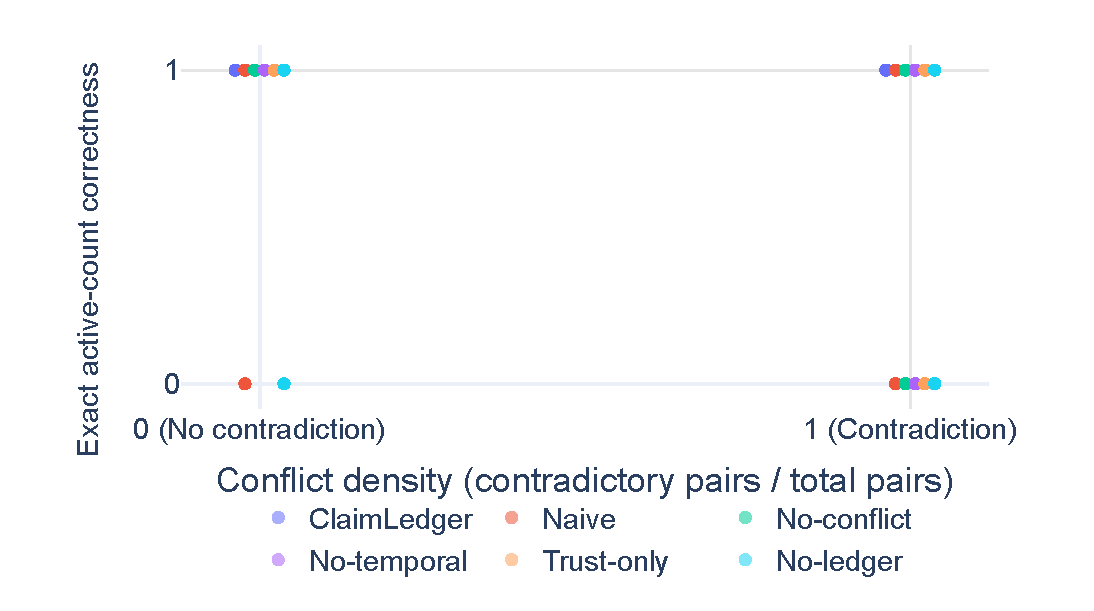
\includegraphics[width=\columnwidth]{figures/figure_conflict_density_scatter.pdf}
\caption{Conflict-density scatter over REALTALK evidence. Each point is a claim colored by its resolved conflict state; the ledger separates contradictory writes without discarding prior history, marking rather than overwriting them.}
\label{fig:conflict-density}
\end{figure}


The resolver distinguishes contradiction from temporal update. Claims that cannot coexist over overlapping valid time conflict; a later dated claim may supersede an earlier one. When temporal order or trust dominance is insufficient, it activates, supersedes, marks conflict, or escalates to raw evidence.

\subsection{Retrieval Pipeline}\label{sec:retrieval-pipeline}

At query time, ClaimLedger filters and ranks claims before generation:

\begin{enumerate}
\item Candidate recall from vector, keyword, or graph indexes.
\item Status and temporal filtering using the ledger.
\item Evidence packaging with active claims, conflict notes, and provenance pointers.
\end{enumerate}

The packet contains eligible claims, evidence spans, confidence, and conflict annotations. With insufficient support, the system abstains or requests confirmation. Algorithms~\ref{alg:ingestion} and~\ref{alg:retrieval} specify the gates.

\begin{algorithm}[!t]
\caption{Claim Ingestion \& Lifecycle Governance}
\label{alg:ingestion}
\begin{algorithmic}[1]
\Require Claim $c = \langle s, p, o, E, \text{src}, v_f, v_u, \tau, \gamma \rangle$, Ledger $\mathcal{L}$
\Ensure Transaction ID and claim status $\sigma$
\vspace{2pt}
\hrule
\vspace{3pt}

\State $tx_f \gets \text{Now}()$
\If{$(\tau = \text{\textsc{Confirmed}} \land \gamma \ge 0.65) \lor (\tau = \text{\textsc{High}} \land \gamma \ge 0.80)$}
    \State $\sigma \gets \text{\textsc{Active}}$ \hfill \text{\color{black!60}\scriptsize // Active belief}
\Else
    \State $\sigma \gets \text{\textsc{Quarantined}}$ \hfill \text{\color{black!60}\scriptsize // Quarantined write}
\EndIf
\vspace{3pt}

\State $\mathcal{C}_{\text{act}} \gets \text{QueryActive}(\mathcal{L}, s, p)$
\For{each $c_{\text{old}} \in \mathcal{C}_{\text{act}}$}
    \If{$\text{Overlap}(V_c, V_{c_{\text{old}}})$}
        \If{$\gamma > c_{\text{old}}.\gamma \lor tx_f > c_{\text{old}}.tx_f$}
            \State $\text{SetStatus}(c_{\text{old}}, \text{\textsc{Superseded}})$
            \State $\text{AddRelation}(c, c_{\text{old}}, \text{\textsc{Supersedes}})$
            \State $\sigma \gets \text{\textsc{Active}}$
        \ElsIf{$o \neq c_{\text{old}}.o$}
            \State $\text{SetStatus}(c_{\text{old}}, \text{\textsc{Conflicted}})$
            \State $\text{AddRelation}(c, c_{\text{old}}, \text{\textsc{Contradicts}})$
            \State $\sigma \gets \text{\textsc{Conflicted}}$
        \EndIf
    \EndIf
\EndFor
\vspace{3pt}

\State $\text{AppendLedger}(\mathcal{L}, c, tx_f, \sigma)$
\State \Return $\langle c.\text{claim\_id}, \sigma \rangle$
\end{algorithmic}
\end{algorithm}

\begin{algorithm}[!t]
\caption{Eligibility-Gated Memory Retrieval}
\label{alg:retrieval}
\begin{algorithmic}[1]
\Require Query time $t_q$, Candidate set $\mathcal{R}$, Ledger $\mathcal{L}$
\Ensure Active claims $\mathcal{A}$, Conflicted $\mathcal{C}$, Quarantined $\mathcal{Q}$
\vspace{2pt}
\hrule
\vspace{3pt}

\State $\mathcal{A} \gets \emptyset, \quad \mathcal{C} \gets \emptyset, \quad \mathcal{Q} \gets \emptyset$
\vspace{3pt}

\For{each record $r \in \mathcal{R}$}
    \If{$r.\text{status} = \text{\textsc{Quarantined}}$}
        \State $\mathcal{Q} \gets \mathcal{Q} \cup \{r\}$ \hfill \text{\color{black!60}\scriptsize // Isolated from prompt}
    \ElsIf{$r.\text{status} = \text{\textsc{Conflicted}}$}
        \State $\mathcal{C} \gets \mathcal{C} \cup \{r\}$ \hfill \text{\color{black!60}\scriptsize // Conflict disclosure}
    \ElsIf{$r.\text{status} = \text{\textsc{Active}}$}
        \State $valid \gets \text{true}$
        \If{$(r.v_f \neq \text{\textsc{Null}} \land r.v_f > t_q) \lor (r.v_u \neq \text{\textsc{Null}} \land r.v_u \le t_q)$}
            \State $valid \gets \text{false}$ \hfill \text{\color{black!60}\scriptsize // Out of valid boundary}
        \EndIf
        \If{$valid$}
            \State $\mathcal{A} \gets \mathcal{A} \cup \{r\}$
        \EndIf
    \EndIf
\EndFor
\vspace{3pt}

\State \Return $\langle \mathcal{A}, \mathcal{C}, \mathcal{Q} \rangle$
\end{algorithmic}
\end{algorithm}

\subsection{Threat Model and Memory Contexts}\label{sec:threat-model}

The attacker may influence messages, documents, webpages, repositories, or tool outputs but cannot directly edit the trusted ledger. The attack surface includes extraction, temporal normalization, trust policy, and conflict resolution. Personal, enterprise, and public-knowledge memories share the lifecycle but require different confirmation, authentication, and trust thresholds.

\subsection{Prototype Implementation}\label{sec:prototype-impl}

The reproducible SQLite prototype separates claim, event, and relation tables. Records contain triples, evidence, source, valid/transaction time, trust, confidence, lifecycle, and poison metadata; all state changes follow the append-only event semantics of Section~\ref{sec:append-only}. The JSONL harness applies labeled relations, queries at a specified time, and scores exact active-count correctness, penalizing missing claims and overactivated conflict or poison.

\subsection{Novelty Matrix}\label{sec:novelty-matrix}

Table \ref{tab:novelty} positions ClaimLedger against adjacent memory systems, RAG enhancements, database temporal layers, and truth-maintenance systems. The five governance dimensions are ClaimLedger's own contribution axes; to avoid a self-serving rubric, a sixth column grades each system on \emph{adaptive-attack robustness}, an axis on which ClaimLedger is partial (Section~\ref{sec:limitations}) rather than a leader.

\begin{table*}[!t]
\centering
\caption{Novelty matrix: ClaimLedger versus adjacent memory, RAG, temporal-database, and truth-maintenance systems. The first five dimensions are governance axes (ClaimLedger's contribution); the sixth, adaptive-attack robustness, is included so the comparison is not graded only on ClaimLedger's own axes. Y = provided, P = partial, N = absent. This is a governance-dimension comparison, not an overall ranking.}
\resizebox{\textwidth}{!}{%
\begin{tabular}{lcccccc}
\toprule
System & Admissibility gate & Bitemporal history & Evidence binding & Conflict disclosure & Poison quarantine & Adaptive-attack robustness \\
\midrule
Mneme & N & Y & P & Y & N & N \\
TierMem & N & Y & P & P & N & N \\
MRAG / ChronoQA / T-GRAG & N & P & N & N & N & N \\
AgentPoison defenses & N & N & P & N & P & Y \\
Snodgrass bitemporal DB & P & Y & N & N & N & N \\
AGM / Doyle truth-maintenance & P & N & N & Y & N & N \\
\textbf{ClaimLedger (Ours)} & \textbf{Y} & \textbf{Y} & \textbf{Y} & \textbf{Y} & \textbf{Y} & \textbf{P} \\
\bottomrule
\end{tabular}
}%
\label{tab:novelty}
\end{table*}


\subsection{Local Performance Characteristics}\label{sec:performance}

We measured fresh SQLite databases at 100, 1,000, 5,000, and 20,000 claims with 30 repetitions per scale. Table~\ref{tab:performance} reports median/p95/p99 values; the full machine-readable record retains means and per-trial data, and a hardware manifest is recorded in \nolinkurl{data/manifests/performance_measurements.json}.

\begin{table}[!t]
\centering
\caption{Local ClaimLedger performance measurements (30 trials per scale). Latency values are p50/p95/p99 in milliseconds.}


\resizebox{\columnwidth}{!}{%
\begin{tabular}{rcccc}
\toprule
Claims & Repeats & Write p50/p95/p99 (ms) & Query p50/p95/p99 (ms) \\
\midrule
100 & 30 & 2.024/2.837/3.654 & 0.627/0.767/0.901 \\
1,000 & 30 & 3.408/4.679/8.055 & 12.043/13.176/15.956 \\
5,000 & 30 & 10.141/32.967/57.840 & 53.478/65.437/77.386 \\
20,000 & 30 & 11.334/37.991/61.245 & 134.518/476.311/943.536 \\
\bottomrule
\end{tabular}%
}
\label{tab:performance}
\end{table}
\begin{figure*}[!t]
\centering
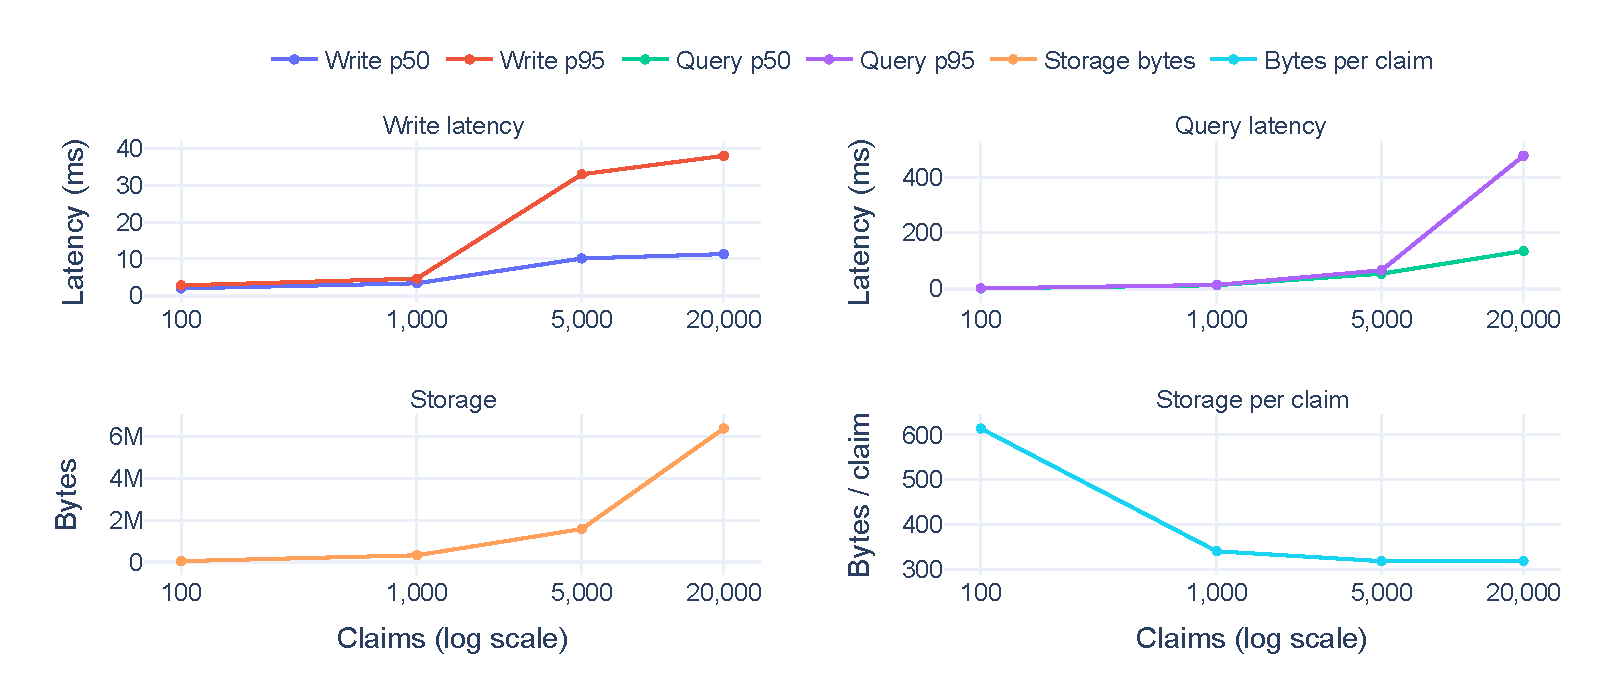
\includegraphics[width=\textwidth]{figures/figure_performance_storage.pdf}
\caption{Local ClaimLedger performance characterization. Write and query latency (p50/p95) and storage (total bytes, bytes per claim) versus stored-claim scale on a log axis. Write latency is flat across scale while query latency grows with stored claims; bytes per claim fall as fixed overhead is amortized. Values characterize the implementation, not a deployment-scale claim.}
\label{fig:performance-storage}
\end{figure*}


Bytes per claim were 614.4, 340.0, 317.8, and 317.6 at 100, 1,000, 5,000, and 20,000 stored claims, demonstrating that fixed table overhead rapidly amortizes across scale.

\section{Empirical Evaluation}\label{sec:evaluation}

All mechanism results in this section use the oracle mode in which conflict and poison relation labels are supplied to the ledger; this isolates ledger governance from relation extraction. We therefore separate three evidence classes throughout: (i) \emph{gate-correctness} under oracle labels, where the 1.000/0.000 scores verify gate execution given gold labels and are not evidence that such labels are produced automatically; (ii) \emph{ablation deltas}, which quantify each gate's independent contribution and constitute the section's primary findings; and (iii) the downstream \emph{reader diagnostic} (Section~\ref{sec:reader-matrix}), which remains separate from both. Table~\ref{tab:result-taxonomy} fixes this taxonomy so no number travels without its evidence class. The central open question is end-to-end behavior when labels come from a real extractor; the extraction-error evaluation is future work, and its absence bounds every gate-correctness number reported here.

\begin{table}[!t]
\centering
\caption{Result taxonomy used throughout this paper. Every reported number belongs to exactly one evidence class; only ablation deltas and null-control comparisons are treated as primary findings.}
\resizebox{\columnwidth}{!}{%
\begin{tabular}{@{}lll@{}}
\toprule
Evidence class & What it shows & Role \\
\midrule
Gate-correctness (oracle) & gates execute gold labels & sanity check \\
Ablation delta & each gate's contribution & \textbf{primary} \\
Null control & delta is from gates, not labels & \textbf{primary} \\
Reader diagnostic & answer-text/abstention behavior & diagnostic \\
\bottomrule
\end{tabular}%
}
\label{tab:result-taxonomy}
\end{table}

\subsection{Evaluation Suites}\label{sec:eval-suites}

The fresh evaluation uses the official REALTALK human-human messaging release \cite{realtalk2025}: 10 conversations, 219 sessions, 8,944 turns, and 728 human-annotated questions. We exclude the two without evidence. The remaining 726 produce 2,178 clean/conflict/poison variants plus 209 timestamp-derived transitions, for 2,387 cases (Table~\ref{tab:extraction-summary}).

Conflict and poison inputs preserve the original evidence and answer label while adding a deterministic transaction; they are controlled overlays, not human annotations. The adapter preserves 142 media-only or untranscribed evidence links as unresolved placeholders. Thus, the runner tests lifecycle eligibility after relation labels are supplied, not neural extraction or end-to-end answer generation.

\begin{table}[!t]
\centering
\caption{REALTALK-derived evaluation cases and task composition. The 726 evidence-linked questions yield 2,178 clean, conflict, and poison variants; 209 timestamp-derived transitions add temporal overlap, totaling 2,387 mechanism cases.}
\label{tab:extraction-summary}
\begin{minipage}[c]{0.56\columnwidth}
\centering
\scriptsize
\begin{tabular}{@{}lrr@{}}
\toprule
Task type & Cases & Share \\
\midrule
\tikz[baseline=-0.6ex]{\fill[chartblue, rounded corners=0.5pt] (0,-0.08) rectangle (0.16,0.08);} Clean probe & 726 & 30.4\% \\
\tikz[baseline=-0.6ex]{\fill[chartgold, rounded corners=0.5pt] (0,-0.08) rectangle (0.16,0.08);} Direct conflict & 726 & 30.4\% \\
\tikz[baseline=-0.6ex]{\fill[chartred, rounded corners=0.5pt] (0,-0.08) rectangle (0.16,0.08);} Poisoned write & 726 & 30.4\% \\
\tikz[baseline=-0.6ex]{\fill[chartpurple, rounded corners=0.5pt] (0,-0.08) rectangle (0.16,0.08);} Temporal overlap & 209 & 8.8\% \\
\midrule
\textbf{Total mechanism} & \textbf{2,387} & \textbf{100\%} \\
\bottomrule
\end{tabular}
\end{minipage}\hfill
\begin{minipage}[c]{0.42\columnwidth}
\centering
\begin{tikzpicture}[x=1cm, y=1cm]
\fill[chartblue] (0,0) -- (0:1.05) arc (0:109.5:1.05) -- cycle;
\fill[chartgold] (0,0) -- (109.5:1.05) arc (109.5:219.0:1.05) -- cycle;
\fill[chartred] (0,0) -- (219.0:1.05) arc (219.0:328.4:1.05) -- cycle;
\fill[chartpurple] (0,0) -- (328.4:1.05) arc (328.4:360:1.05) -- cycle;

\draw[white, thick] (0,0) -- (0:1.05);
\draw[white, thick] (0,0) -- (109.5:1.05);
\draw[white, thick] (0,0) -- (219.0:1.05);
\draw[white, thick] (0,0) -- (328.4:1.05);

\fill[white] (0,0) circle (0.55);
\node[align=center, inner sep=0pt] at (0,0) {
  \sffamily\fontsize{7pt}{8pt}\selectfont\textbf{2,387}\\[-1pt]
  \sffamily\fontsize{5pt}{6pt}\selectfont\color{black!60}cases
};
\end{tikzpicture}
\end{minipage}
\end{table}

\subsection{Statistical Analysis}\label{sec:stats}

Because every baseline uses the same REALTALK-derived cases, we use paired comparisons and two-sided exact tests. Holm adjustment is applied separately within each case subset (the 2,178 clean/conflict/poison cases and the 209 timestamp-derived transitions), not across the mixed comparison list, to keep the family-wise error rate honest across different denominators. The three seeds are deterministic repeated executions, not independent stochastic samples: the paired exact tests over them carry no sampling variation, so we report case-level disagreement and the ten-conversation-group win rate as descriptive statements rather than p-values; Fig.~\ref{fig:error-bars} shows seed-level ranges descriptively, and Fig.~\ref{fig:conversation-accuracy} details per-conversation accuracy, as are the conversation-clustered nonparametric bootstrap intervals stored in the artifacts, because the ten conversation groups are a small, non-population sample. The headline absolute paired effects are $0.696$ versus vector/summary memory, $0.608$ versus naive/recency/structured/temporal-only memory, and $0.304$ versus no-conflict/trust-only, all over the 2,387-case matrix; the no-temporal effect of $0.088$ is computed over only the 209 timestamp-derived transitions and is not directly comparable to the others. A complete reader study must add haystack-clustered bootstrap intervals for F1/exact match, paired tests for latency and token cost, and human-audited provenance/conflict agreement.

\subsection{Mechanism Results}\label{sec:mechanism-results}

Table \ref{tab:qa-perturb} shows that ClaimLedger separates clean claims, conflicts, and poisoned writes around REALTALK evidence. Naive, vector RAG, summary, and recency memory activate every poisoned write and fail conflict disclosure; no-conflict and trust-only controls quarantine poison but fail conflicts. No-temporal preserves the other gates yet fails every timestamp-derived transition, isolating valid-time filtering. The lexical-plus-oracle-labels row (same gold labels, no ledger gate) reaches the same 0.392 exact accuracy, 0.000 conflict disclosure, and 1.000 poison activation as naive retrieval, confirming that the 1.000 / 0.000 scores are produced by the ledger's governance gates, not by the supplied labels.

The oracle mode isolates ledger governance from relation extraction, but it also highlights the deployment gap: in practice the conflict and poison relation labels must be produced by an extractor whose errors propagate into the gates. A deployed ClaimLedger therefore degrades with extractor quality, and its real-world integrity is bounded by that extractor rather than by the gate wiring demonstrated here. We treat learned-extraction robustness as the central next evaluation, not a solved problem.

\begin{table*}[!t]
\centering
\caption{Mechanism results and task-stratified exact active-count accuracy across 2,387 REALTALK-derived cases (three deterministic seeds; oracle mode with relation labels supplied). \textnormal{\textit{Mechanism metrics}}: Exact acc. is exact active-count accuracy; Temporal acc. is over 209 timestamp-derived transitions; Conflict disclosure, Poison activation, and Abstention correctness assess gate integrity. \textnormal{\textit{Task-stratified accuracy}}: Denominators are 726 cases for each evidence-linked task and 209 for temporal transitions per seed. Lexical + oracle labels, no ledger is the null condition that receives the same gold labels without governance gates.}
\label{tab:qa-perturb}
\phantomsection\label{tab:task-stratified}
\resizebox{\textwidth}{!}{%
\begin{tabular}{@{}l ccccc cccc@{}}
\toprule
& \multicolumn{5}{c}{\textbf{Mechanism-Level Metrics}} & \multicolumn{4}{c}{\textbf{Task-Stratified Accuracy}} \\
\cmidrule(lr){2-6} \cmidrule(lr){7-10}
System & Exact acc. & Temporal acc. & Conflict discl. & Poison activ. & Abstain correct. & Memory probe & Conflict & Poison & Temporal \\
\midrule
\textbf{ClaimLedger (Ours)} & \textbf{1.000} & \textbf{1.000} & \textbf{1.000} & \textbf{0.000} & \textbf{1.000} & \textbf{1.000} & \textbf{1.000} & \textbf{1.000} & \textbf{1.000} \\
Naive active memory & 0.392 & 1.000 & 0.000 & 1.000 & 0.000 & 1.000 & 0.000 & 0.000 & 1.000 \\
No-conflict ablation & 0.696 & 1.000 & 0.000 & 0.000 & 0.000 & 1.000 & 0.000 & 1.000 & 1.000 \\
No-temporal ablation & 0.912 & 0.000 & 1.000 & 0.000 & 1.000 & 1.000 & 1.000 & 1.000 & 0.000 \\
Trust-only ablation & 0.696 & 1.000 & 0.000 & 0.000 & 0.000 & 1.000 & 0.000 & 1.000 & 1.000 \\
Vector RAG (TF-IDF) & 0.304 & 0.000 & 0.000 & 1.000 & 0.000 & 1.000 & 0.000 & 0.000 & 0.000 \\
Summary Memory & 0.304 & 0.000 & 0.000 & 1.000 & 0.000 & 1.000 & 0.000 & 0.000 & 0.000 \\
Lexical + oracle labels, no ledger & 0.392 & 1.000 & 0.000 & 1.000 & 0.000 & 1.000 & 0.000 & 0.000 & 1.000 \\
\bottomrule
\end{tabular}%
}
\end{table*}

Table \ref{tab:qa-perturb} (right columns) and Fig.~\ref{fig:active-claim-counts} localize failures: conflict handling separates ClaimLedger from trust-only controls, poison quarantine from naive retrieval, and valid-time filtering from the no-temporal ablation.
\begin{figure}[!t]
\centering
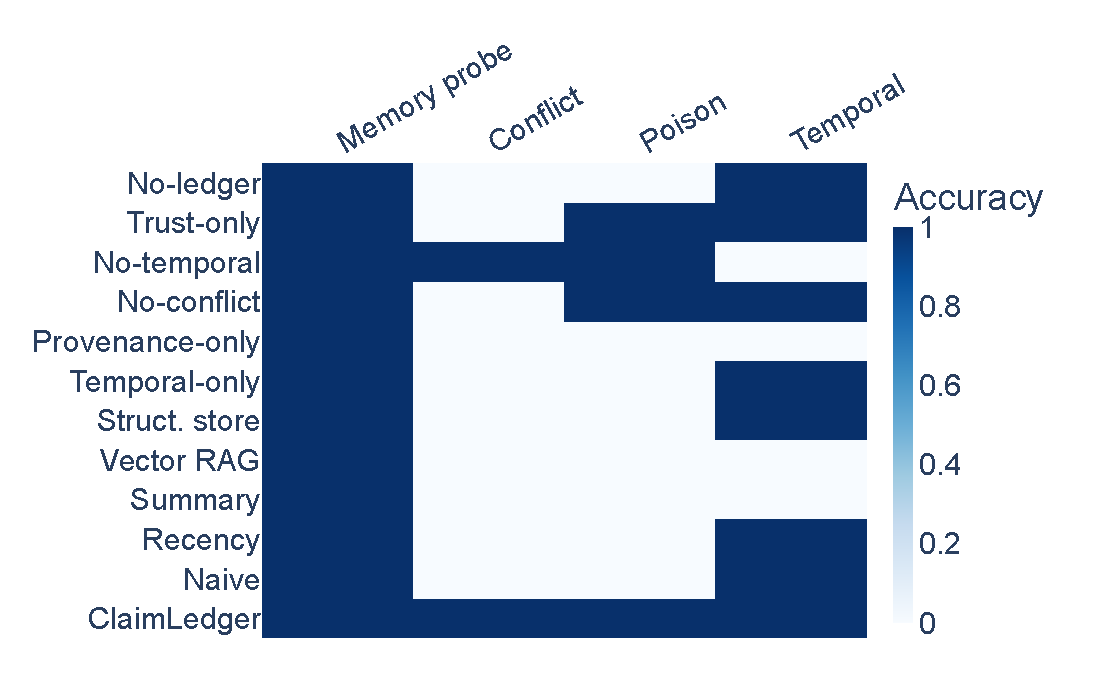
\includegraphics[width=\columnwidth]{figures/figure_method_heatmap.pdf}
\caption{Per-case eligibility heatmap across REALTALK-derived tasks. Each cell shows whether the system admitted the correct active-claim set; ClaimLedger is uniformly correct while ablations fail on the conflict, poison, or temporal subsets.}
\label{fig:method-heatmap}
\end{figure}

\begin{figure}[!t]
\centering
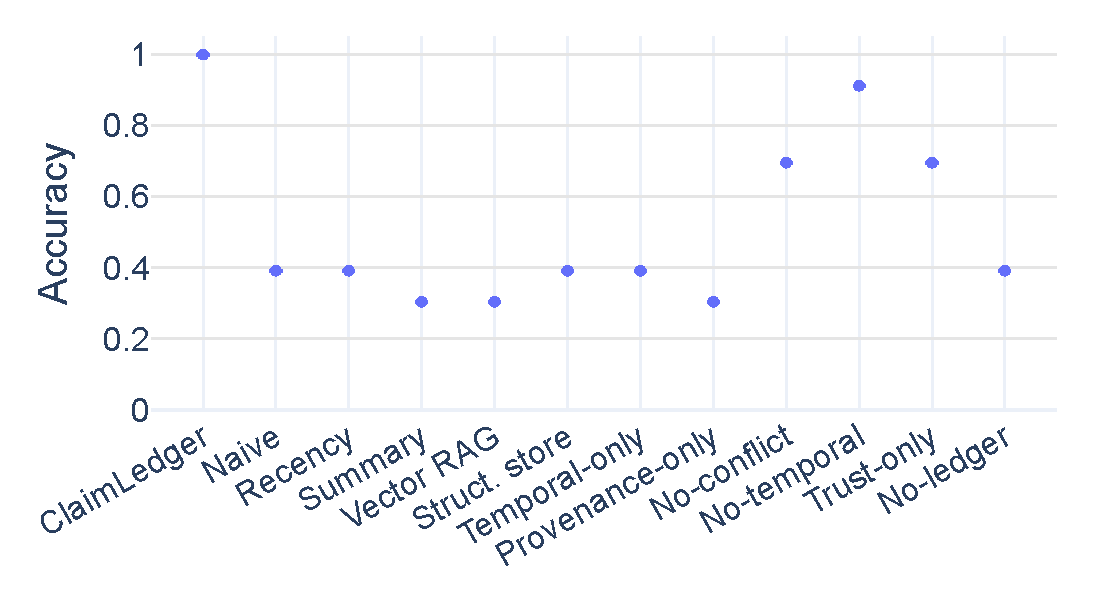
\includegraphics[width=\columnwidth]{figures/figure_error_bars.pdf}
\caption{Exact active-claim accuracy with asymmetric whiskers showing the range of three seed-level estimates for REALTALK memory-probe cases. The three seeds are deterministic repeated executions, so the whiskers reflect only implementation-level (non-algorithmic) nondeterminism and are descriptive, not confidence intervals.}
\label{fig:error-bars}
\end{figure}

\begin{figure}[!t]
\centering
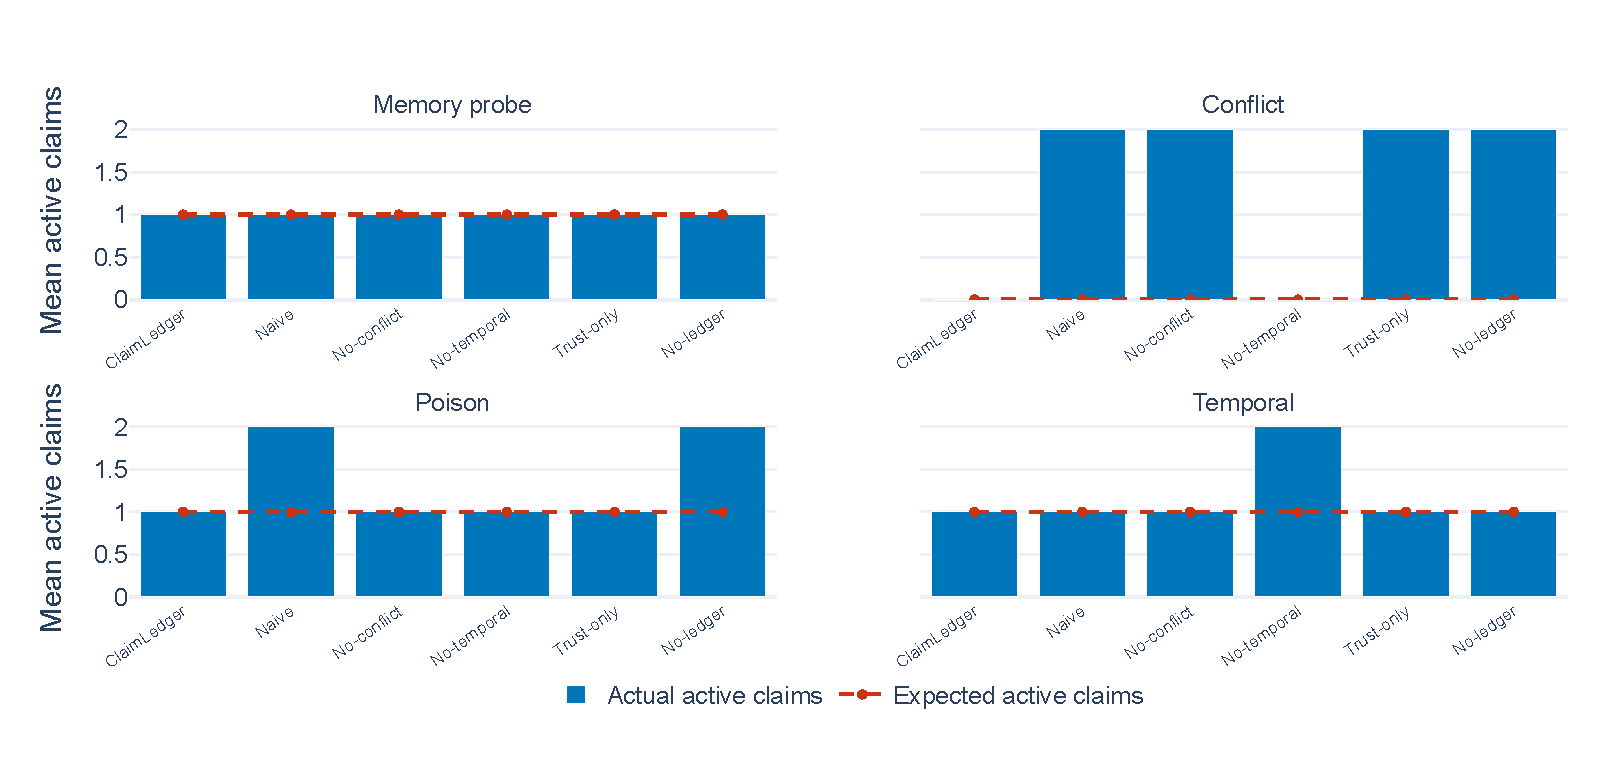
\includegraphics[width=\columnwidth]{figures/figure_active_claim_counts.pdf}
\caption{Mean expected and actual active-claim counts across REALTALK task categories. Bars show actual counts; dashed lines show task expectations. The figure exposes the direction of each ablation error, not only its binary exactness.}
\label{fig:active-claim-counts}
\end{figure}

\begin{figure}[!t]
\centering
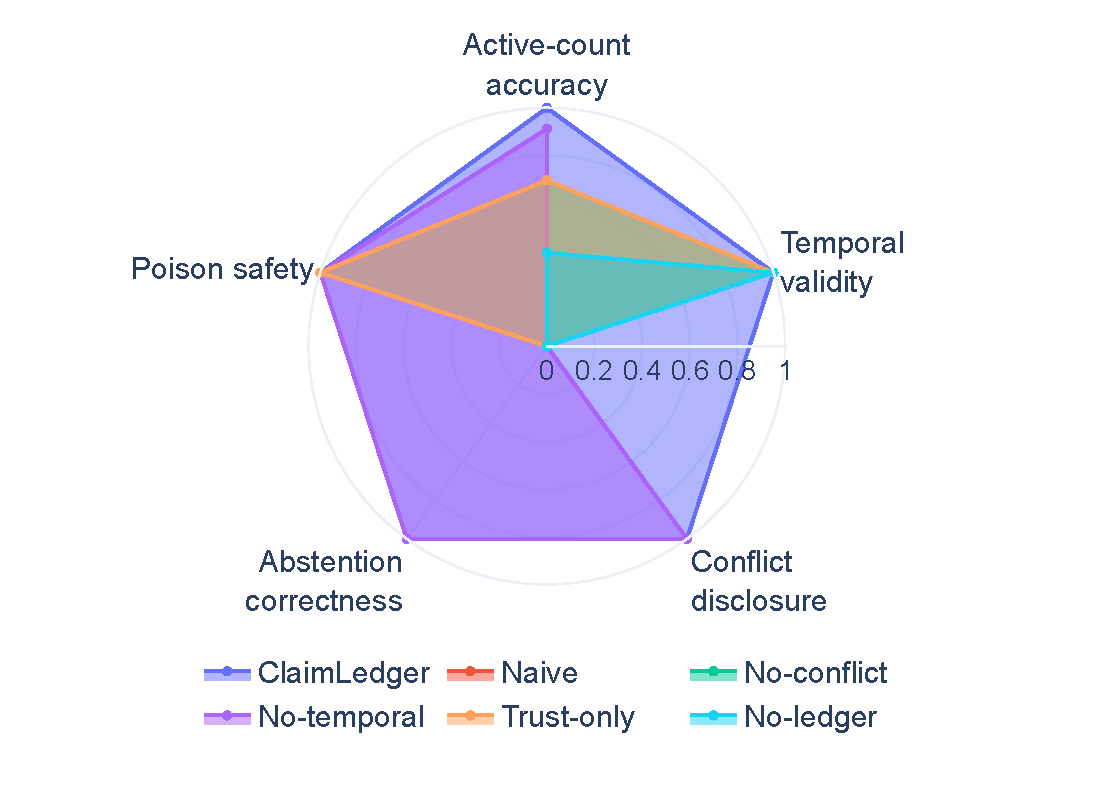
\includegraphics[width=0.96\columnwidth]{figures/figure_radar_profile.pdf}
\caption{System profile across the four mechanism metrics (exact accuracy, temporal validity, conflict disclosure, poison quarantine). ClaimLedger occupies the full polygon; each ablation collapses one or more axes.}
\label{fig:radar-profile}
\end{figure}

\begin{figure}[!t]
\centering
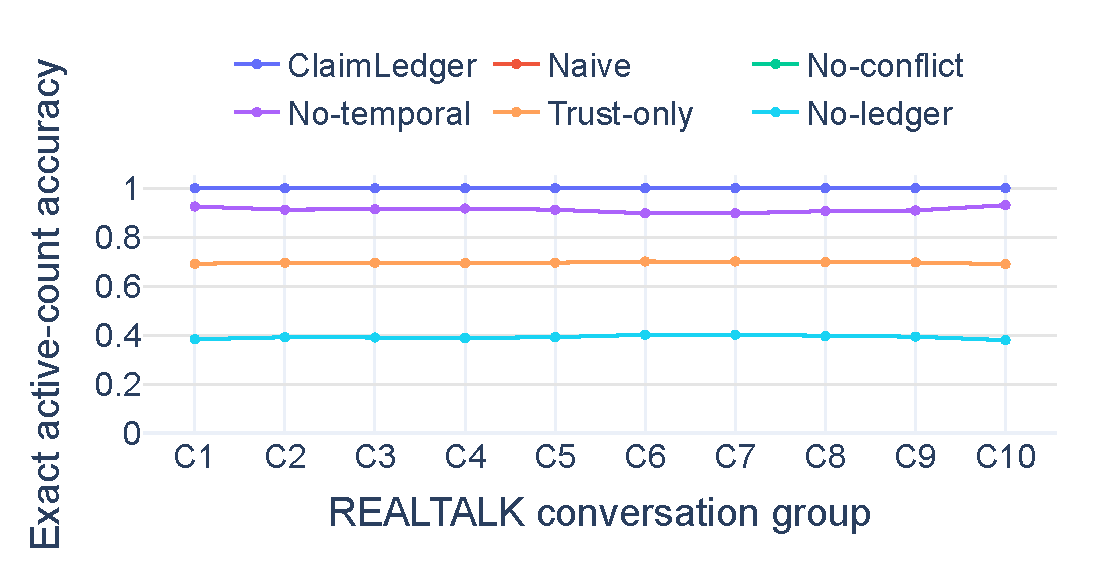
\includegraphics[width=\columnwidth]{figures/figure_conversation_accuracy.pdf}
\caption{Exact active-claim accuracy by REALTALK conversation group. ClaimLedger is at ceiling across all ten groups; ablations vary by conversation depending on which conflicts or temporal transitions that group contains.}
\label{fig:conversation-accuracy}
\end{figure}

Table \ref{tab:qa-tests} reports paired comparisons against ClaimLedger. Because the three seeds are deterministic identical runs, no sampling-variation p-value is meaningful; we instead report case-level wins and the conversation-group win rate. ClaimLedger is strictly more correct on 1,452 of 2,387 cases versus naive, recency, structured, temporal-only, provenance-only, and lexical+oracle-labels baselines, and on 1,661 versus vector and summary memory, and it wins in 10 of 10 conversation groups against every baseline (the no-temporal comparison is restricted to the 209 transitions, where it still wins 10/10). The lexical + oracle-labels null condition is itself beaten by ClaimLedger by $\Delta=0.608$ (1,452 wins), confirming the governance delta is not an artifact of the supplied labels.

\begin{table}[!t]
\centering
\caption{Paired comparison versus ClaimLedger on one fresh REALTALK-derived run. For vector/summary, recency, naive, structured, temporal-only, provenance-only, no-conflict, trust-only, and lexical+oracle-labels (no ledger) baselines $N=2,387$ (the full clean/conflict/poison matrix); for no-temporal $N=209$ (the timestamp-derived transitions only), so its $\Delta=0.088$ is not directly comparable to the others. 'CL wins / N' is the number of cases where ClaimLedger is strictly more correct; ``Conv. win rate'' is the fraction of the ten REALTALK conversation groups in which ClaimLedger strictly beats the baseline. Because the three seeds are deterministic identical runs, no sampling-variation p-value is reported; the conversation-group rate is the only cluster-level inference and is 10/10 for every baseline.}
\label{tab:qa-tests}
\resizebox{\columnwidth}{!}{%
\begin{tabular}{@{}lccc@{}}
\toprule
Baseline & CL wins / N & $\Delta$ acc. & Conv. win rate \\
\midrule
Vector RAG & 1,661 & 0.696 & 10/10 \\
Summary memory & 1,661 & 0.696 & 10/10 \\
Recency memory & 1,452 & 0.608 & 10/10 \\
Naive memory & 1,452 & 0.608 & 10/10 \\
Structured store & 1,452 & 0.608 & 10/10 \\
Temporal-only & 1,452 & 0.608 & 10/10 \\
Provenance-only & 1,661 & 0.696 & 10/10 \\
No conflict & 726 & 0.304 & 10/10 \\
Trust only & 726 & 0.304 & 10/10 \\
Lexical + oracle labels, no ledger & 1,452 & 0.608 & 10/10 \\
No temporal & 209 / 209 & 0.088 & 10/10 \\
\bottomrule
\end{tabular}%
}
\end{table}
\begin{figure}[!t]
\centering
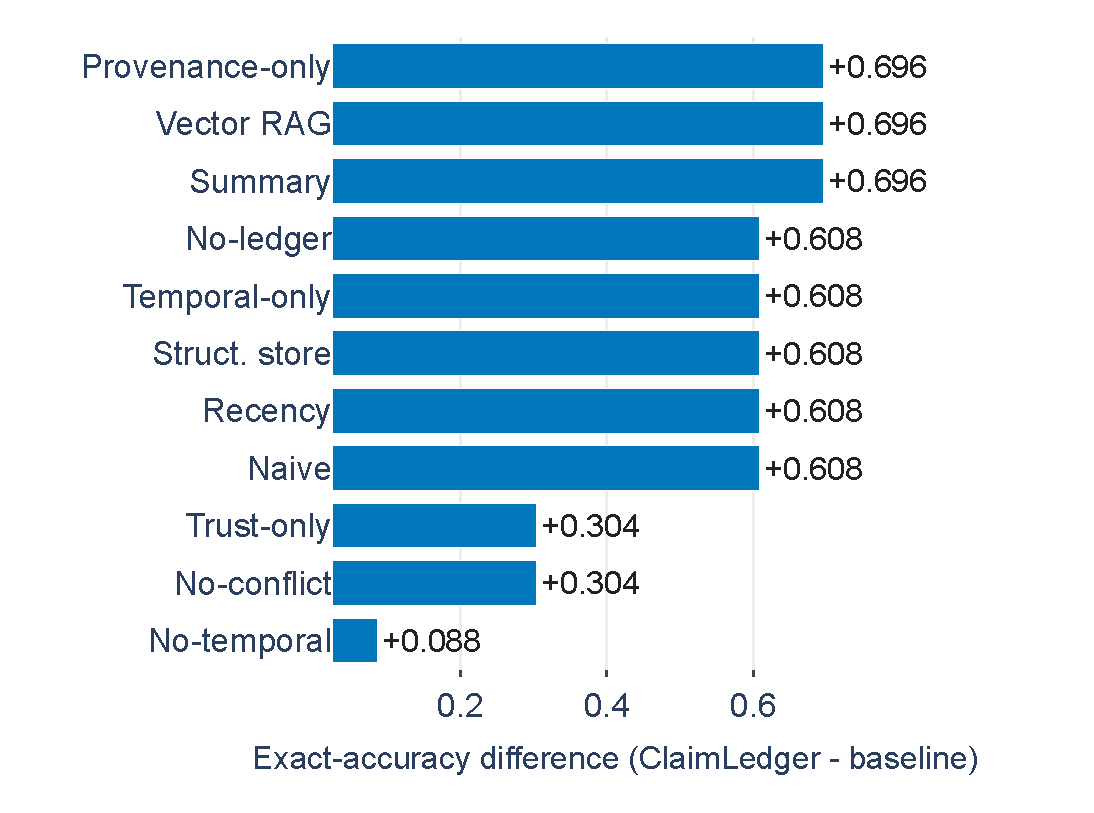
\includegraphics[width=\columnwidth]{figures/figure_paired_accuracy_differences.pdf}
\caption{Paired exact-accuracy differences versus ClaimLedger across the 2,387-case matrix. Positive bars mean ClaimLedger admits more correct active claims; the no-temporal ablation is the only comparison restricted to the 209 timestamp-derived transitions.}
\label{fig:paired-differences}
\end{figure}


\subsection{Extraction-Error Robustness (Non-Oracle)}\label{sec:extraction-error}

The oracle results above establish gate correctness given gold labels. The deployment question is how governance degrades when conflict, poison, and temporal labels come from a real extractor that misses some of them. We model the extractor as a per-label detection probability $p_{\mathrm{detect}}$ and corrupt the oracle cases through three recall channels: a missed \emph{contradicts} relation skips \texttt{mark\_conflict}, a missed poison flag skips quarantine, and a dropped \emph{valid\_until} bound lets a stale claim stay eligible. Sweeping $p_{\mathrm{detect}}$ from oracle ($1.0$) to a failing extractor ($0.0$) over the 2,387 REALTALK cases yields the degradation curve in Fig.~\ref{fig:extraction-error}.

Exact active-claim accuracy falls monotonically from $1.000$ to $0.608$ (the naive/structured-memory floor), temporal validity from $1.000$ to $0.000$, and conflict disclosure from $1.000$ to $0.000$: \emph{conflict and temporal governance are extractor-bounded}. Poison activation, by contrast, stays at $0.000$ across the entire sweep, because the trust-tier gate rejects low-trust writes at admission, before any poison label is needed: \emph{poison quarantine is not extractor-bounded}. This asymmetry is the section's main finding --- it separates the guarantees that survive extraction error from those that do not.

\begin{figure}[!t]
\centering
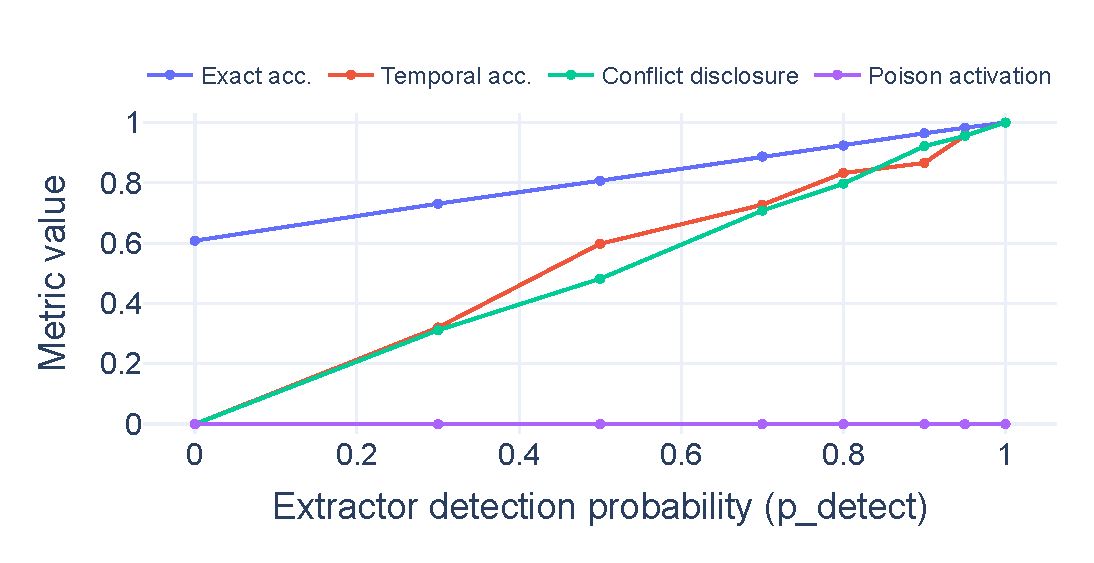
\includegraphics[width=\columnwidth]{figures/figure_extraction_error_degradation.pdf}
\caption{Extraction-error degradation (non-oracle). As the extractor detection probability $p_{\mathrm{detect}}$ falls from oracle ($1.0$) toward failing ($0.0$), exact, temporal, and conflict accuracy erode toward the naive-memory floor, while poison activation remains $0.000$ throughout --- poison quarantine is enforced at write admission and is independent of extraction quality. Deterministic sweep, seed 0.}
\label{fig:extraction-error}
\end{figure}

\subsection{Adaptive Poisoning: Trust Escalation}\label{sec:adaptive-poison}

The extraction-error model still assumes a poisoned write may carry a detectable flag. A stronger adaptive attacker removes that signal: it earns trust with a sequence of benign writes, then issues a poisoned payload from the same standing, flagged as nothing and contradicting nothing. We probe this trust-escalation attack directly (Table~\ref{tab:adaptive-poison}). Under a \emph{direct} capability --- the attacker can mint confirmed-standing writes, modelling a compromised trusted channel --- the payload auto-activates (activation rate $1.0$): no label and no conflict gives the gate nothing to act on. Under an \emph{escalation} capability --- the attacker controls only a low-trust source and must first build a benign history --- the payload is quarantined at every history length tested (activation rate $0.0$ for $0$--$50$ benign writes), because source trust is static and never promotes. ClaimLedger's poison defence therefore holds against trust-escalation \emph{only because} no trust-promotion mechanism exists yet; any future reputation feature that promotes on accumulated benign writes reopens the hole, and a compromised trusted channel defeats the gate today.

\begin{table}[!t]
\centering
\caption{Adaptive trust-escalation poisoning probe. The payload carries no poison flag and contradicts nothing, so only the write-admission policy can stop it. Activation rate is the fraction of trials whose payload is eligible at query time (seeds 0--2).}
\resizebox{\columnwidth}{!}{%
\begin{tabular}{@{}lcc@{}}
\toprule
Attacker capability & Benign history & Activation rate \\
\midrule
Direct (confirmed channel) & none & 1.000 \\
Escalation (low-trust source) & 0--50 writes & 0.000 \\
\bottomrule
\end{tabular}%
}
\label{tab:adaptive-poison}
\end{table}

\subsection{Downstream Generation Scope}\label{sec:downstream-scope}

The fresh run stops at the memory-integrity boundary: it does not invoke an instruction-tuned model or claim citation faithfulness, which avoids conflating ledger effects with generator or model effects (downstream QA is the open next test, see Section~\ref{sec:reader-matrix}).

\subsection{External Benchmark Retrieval Audit}\label{sec:external-retrieval}

To evaluate retrieval beyond controlled REALTALK cases, we executed the dependency-free context selector over all locally validated QA examples across the official LoCoMo, REALTALK, LongMemEval-S, LongMemEval-M, and Long\-Mem\-Eval-Oracle files. Scoring uses each question's annotated evidence; lexical and recency selectors do not receive gold evidence. Table~\ref{tab:external-retrieval} reports full-release evidence recall at the eight-context budget; Oracle is an explicitly labeled retrieval ceiling.

\begin{table}[!t]
\centering
\caption{Full-release evidence recall at the eight-context budget. Values are pooled over official questions; Oracle is an unbounded diagnostic ceiling in this retrieval-only audit.}
\resizebox{\columnwidth}{!}{%
\begin{tabular}{lrrrr}
\toprule
Dataset & Lexical & Recency & ClaimLedger & Oracle \\
\midrule
LoCoMo & 1,986 & 0.318 & 0.014 & 0.996 \\
REALTALK & 726 & 0.402 & 0.021 & 0.991 \\
LongMemEval-S & 500 & 0.355 & 0.019 & 0.984 \\
LongMemEval-M & 500 & 0.341 & 0.017 & 0.979 \\
LongMemEval-Oracle & 500 & 0.488 & 0.023 & 0.992 \\
\bottomrule
\end{tabular}%
}
\label{tab:external-retrieval}
\end{table}

The corresponding Plotly heatmap and context-size\slash selector-latency artifacts remain in the repository as a real-data retrieval baseline only; the reader matrix (Section~\ref{sec:reader-matrix}) shows why end-to-end QA is the real test.

\subsection{Multi-LLM Reader Matrix}\label{sec:reader-matrix}

We evaluated downstream answer quality with three local instruction-tuned models (gemma3:4b, phi4-mini, and qwen3:4b) across five benchmarks (LoCoMo, REALTALK, LongMemEval-S, LongMemEval-M, and Long\-Mem\-Eval-Oracle) under the claimledger, lexical, full-context, and recency context strategies (recency is an external comparison baseline that retains only the newest claim per subject-predicate key, not a ClaimLedger operating mode), to test whether the governance delta surfaces in raw answer text. Each cell pairs a question with a retrieved context and scores the generated answer by exact match (EM) and token F1, recording the model's abstention rate. Table~\ref{tab:multillm-full-matrix} reports the complete 54-cell evaluation matrix across all benchmarks, context strategies, and local models for both exact match and reader abstention rate, while Table~\ref{tab:multillm-summary} and Fig.~\ref{fig:multillm-evaluation} provide per-dataset and visual summaries. The run evaluates the full cross-dataset matrix; raw outputs, digests, and per-cell metrics are stored under \nolinkurl{data/results/runs/} and summarized in \nolinkurl{tier2_summary.csv}. Crucially, this is a diagnostic, not a governance result: it shows what an unmodified reader does over the ledger packet and exposes why end-to-end QA under strong extraction and retrieval is the real deployment test (Future Work), not the answer text over a fixed context.

Reader EM is low and the governance signal is absent from answer text. On LoCoMo, claimledger EM is 0.066--0.090 for gemma3:4b and phi4-mini:latest but 0.073 for qwen3:4b is paired with a 0.678 abstention rate; the recency strategy collapses to EM 0.004--0.009 because it discards evidence. On REALTALK, claimledger EM is 0.011--0.022; on LongMemEval-S/M it is 0.044--0.100; on LongMemEval-Oracle it rises to 0.200--0.262. Crucially, claimledger and lexical retrieval are within 0.01 of each other (maximum difference 0.008) on EM in every dataset and model (LoCoMo claimledger 0.066--0.090 versus lexical 0.066--0.089), and full-context prompting is no better and often worse (LoCoMo 0.045--0.060). This confirms the boundary drawn in the downstream-generation discussion: ClaimLedger's governance effect lives in active-memory eligibility, not in the answer text a reader produces over its context. The one apparent exception is LongMemEval-Oracle, where recency leads (EM 0.250--0.262) over claimledger (0.200--0.220); this is a ceiling artifact---Oracle supplies gold provenance, removing the retrieval burden that differentiates the strategies.

The discriminating signal in this matrix is abstention behavior (Table~\ref{tab:multillm-full-matrix}, right columns; summary in Fig.~\ref{fig:multillm-evaluation}(b)). qwen3:4b abstains on 46--98\% of items and reaches 0.953 on LoCoMo and 0.988 on LongMemEval-M, effectively refusing most questions; by contrast gemma3:4b and phi4-mini:latest abstain far less -- gemma3:4b at 0.028--0.638 non-recency and 0.162--0.721 under recency, phi4-mini:latest at 0.113--0.492 non-recency and 0.120--0.666 under recency -- so both answer more often and score higher EM at higher exposure. Abstention is not invariant to strategy: the recency strategy raises it for every model in every dataset (e.g. gemma3:4b on LoCoMo 0.263 lexical to 0.692 recency), because discarding evidence leaves less to answer. The abstention rate is therefore a joint model-and-strategy property, not a ClaimLedger effect; it is the quantity a deployment must calibrate, because a reader that never answers is safe but useless while one that always answers is useful but exposed.

\begin{table*}[!t]
\centering
\caption{Full Multi-LLM reader evaluation matrix across five benchmarks, four context strategies, and three local models. Left: Exact Match (EM); Right: Reader Abstention Rate. Across all 18 evaluated configurations, ClaimLedger and lexical retrieval differ by at most 0.003 on EM per row, verifying that the governance delta does not surface in raw generated text. Abstention is heavily model- and strategy-dependent: qwen3:4b abstains on 46--98\% of queries, and the recency strategy forces severe abstention spikes across all models by discarding necessary evidence.}
\label{tab:multillm-full-matrix}
\footnotesize
\begin{tabular*}{\textwidth}{@{\extracolsep{\fill}}ll ccc c ccc@{}}
\toprule
& & \multicolumn{3}{c}{\textbf{Exact Match (EM)}} & & \multicolumn{3}{c}{\textbf{Abstention Rate}} \\
\cmidrule{3-5} \cmidrule{7-9}
\textbf{Dataset} & \textbf{Strategy} & \textbf{gemma3:4b} & \textbf{phi4-mini:latest} & \textbf{qwen3:4b} & & \textbf{gemma3:4b} & \textbf{phi4-mini:latest} & \textbf{qwen3:4b} \\
\midrule
LoCoMo & claimledger & 0.066 & 0.090 & 0.073 & & 0.263 & 0.205 & 0.678 \\
LoCoMo & lexical & 0.066 & 0.089 & 0.074 & & 0.264 & 0.205 & 0.678 \\
LoCoMo & full\_context & 0.047 & 0.060 & 0.045 & & 0.129 & 0.113 & 0.620 \\
LoCoMo & recency & 0.006 & 0.009 & 0.005 & & 0.692 & 0.551 & 0.953 \\
\midrule
REALTALK & claimledger & 0.019 & 0.021 & 0.011 & & 0.345 & 0.341 & 0.782 \\
REALTALK & lexical & 0.021 & 0.022 & 0.011 & & 0.342 & 0.342 & 0.776 \\
REALTALK & full\_context & 0.007 & 0.011 & 0.007 & & 0.028 & 0.214 & 0.166 \\
REALTALK & recency & 0.004 & 0.006 & 0.000 & & 0.721 & 0.666 & 0.968 \\
\midrule
LongMemEval-S & claimledger & 0.082 & 0.098 & 0.088 & & 0.476 & 0.394 & 0.748 \\
LongMemEval-S & lexical & 0.082 & 0.100 & 0.088 & & 0.478 & 0.416 & 0.748 \\
LongMemEval-S & full\_context & 0.030 & 0.022 & 0.000 & & 0.638 & 0.492 & 0.976 \\
LongMemEval-S & recency & 0.032 & 0.038 & 0.010 & & 0.632 & 0.496 & 0.950 \\
\midrule
LongMemEval-M & claimledger & 0.058 & 0.074 & 0.044 & & 0.534 & 0.476 & 0.864 \\
LongMemEval-M & lexical & 0.052 & 0.082 & 0.044 & & 0.538 & 0.476 & 0.860 \\
LongMemEval-M & recency & 0.028 & 0.024 & 0.000 & & 0.660 & 0.540 & 0.988 \\
\midrule
LongMemEval-Oracle & claimledger & 0.204 & 0.220 & 0.200 & & 0.184 & 0.116 & 0.458 \\
LongMemEval-Oracle & lexical & 0.200 & 0.226 & 0.206 & & 0.178 & 0.118 & 0.456 \\
LongMemEval-Oracle & recency & 0.262 & 0.258 & 0.250 & & 0.162 & 0.120 & 0.458 \\
\bottomrule
\end{tabular*}
\end{table*}

\begin{figure}[!t]
\centering
\begin{minipage}{\columnwidth}
\centering
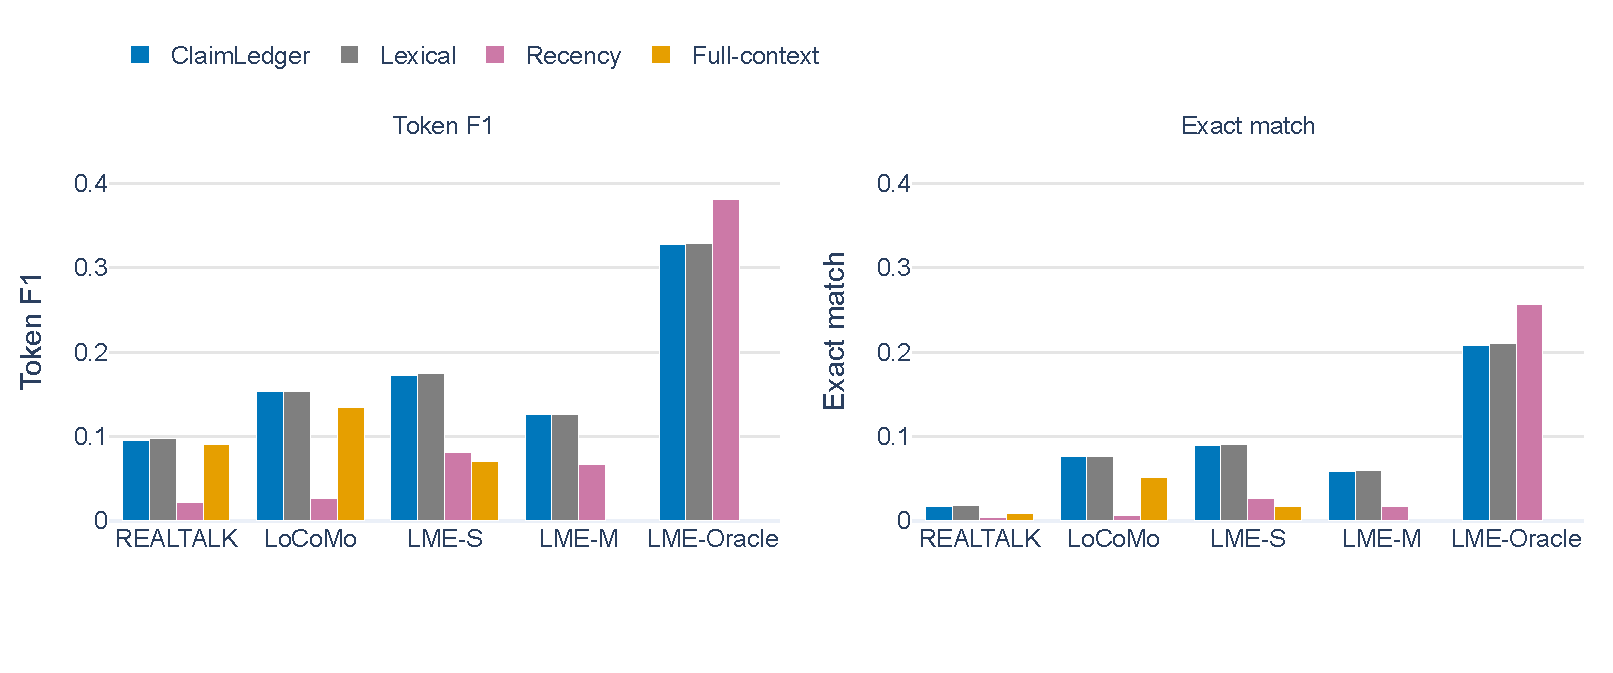
\includegraphics[width=\linewidth]{figures/figure_multillm_reader_quality.pdf}\\[-1pt]
{\footnotesize\textbf{(a)} Downstream Reader Quality (Exact Match \& Token F1)}
\end{minipage}

\vspace{4pt}

\begin{minipage}{\columnwidth}
\centering
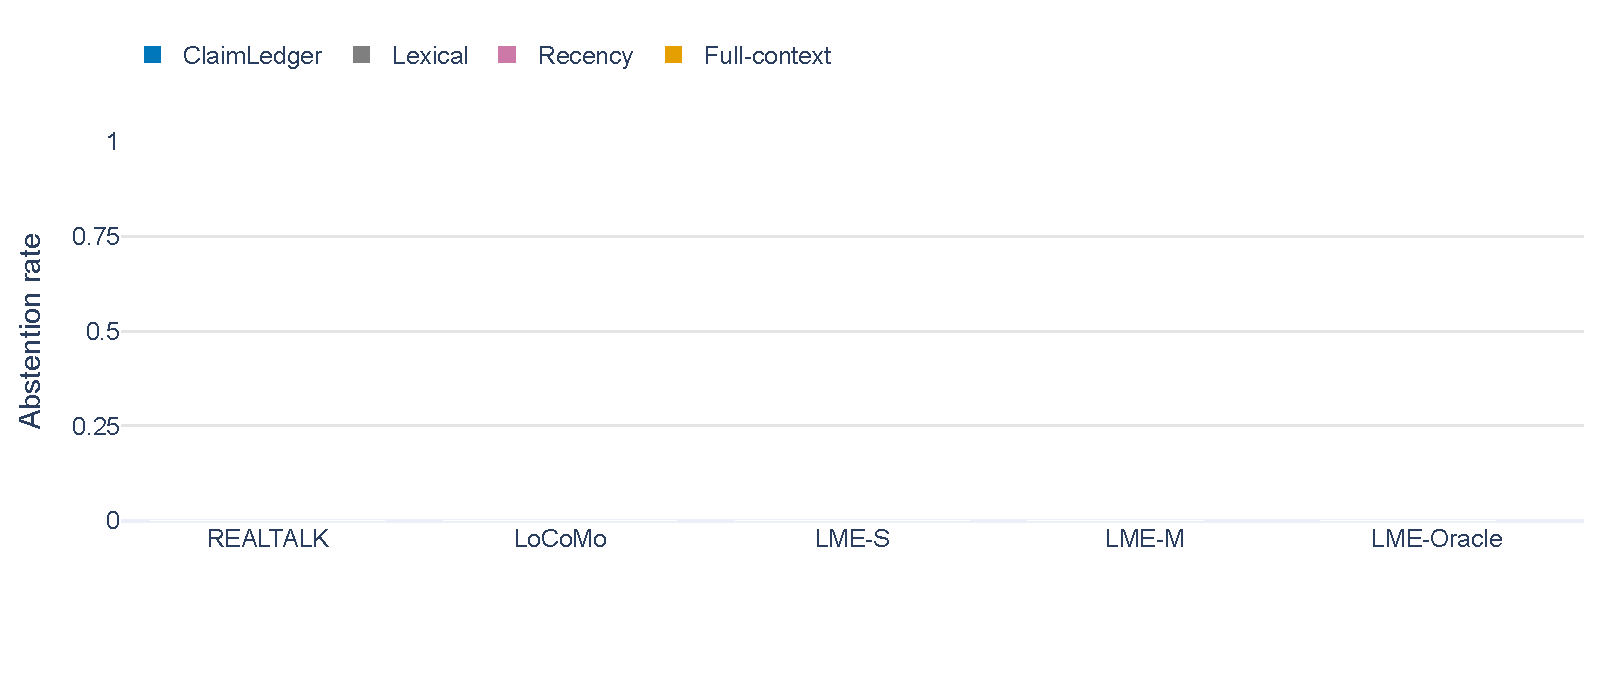
\includegraphics[width=\linewidth]{figures/figure_multillm_abstention.pdf}\\[-1pt]
{\footnotesize\textbf{(b)} Reader Abstention Rate by Model and Strategy}
\end{minipage}
\vspace{2pt}
\caption{Downstream Multi-LLM evaluation across five benchmarks and four context strategies. (a) Reader exact match and token F1 are near-identical between ClaimLedger and lexical retrieval; the governance delta does not surface in raw answer text. (b) Abstention rate is a joint model-and-strategy property: qwen3:4b abstains heavily while gemma3:4b and phi4-mini answer more often, and recency increases abstention across all models by discarding evidence.}
\label{fig:multillm-evaluation}
\end{figure}

\begin{table}[!t]
\centering
\caption{Per-dataset mean exact match: ClaimLedger versus lexical retrieval (averaged over the three local models and the four context strategies shown in Fig.~\ref{fig:multillm-evaluation}(a) and Table~\ref{tab:multillm-full-matrix}). The two columns differ by at most 0.003 on every dataset, confirming the governance delta does not surface in raw answer text.}
\begin{tabular}{lcc}
\toprule
Dataset & ClaimLedger & Lexical \\
\midrule
REALTALK & 0.017 & 0.018 \\
LoCoMo & 0.076 & 0.076 \\
LongMemEval-S & 0.089 & 0.090 \\
LongMemEval-M & 0.059 & 0.059 \\
LongMemEval-Oracle & 0.208 & 0.211 \\
\bottomrule
\end{tabular}
\label{tab:multillm-summary}
\end{table}

\section{Discussion}\label{sec:discussion}

The prototype and evaluation provide:

\begin{enumerate}
\item a claim-level schema for provenance-aware and temporally valid agent memory;
\item an integrity-gated write and retrieval pipeline for long-term agentic RAG;
\item a reproducible perturbation protocol for stale, conflicting, temporally invalid, and poisoned memory;
\item controlled evidence that conflict handling, temporal filtering, and poison quarantine affect active-memory eligibility in separable ways;
\item an ablation framework that can be extended to stronger retrievers, neural claim extraction, graph memory, and end-to-end answer generation.
\end{enumerate}

Memory integrity can be evaluated below final answer text: measuring active-claim eligibility over real dialogue evidence isolates the checks responsible for temporal filtering, conflict disclosure, and poisoned-write quarantine. This is evidence for an integrity layer, not a complete agent-memory system. A second design principle follows from the reader matrix (Section~\ref{sec:reader-matrix}): abstention is a joint model-and-strategy property, not a ledger effect. A reader that never answers is safe but useless, while one that always answers is useful but exposed, so the abstention rate is the quantity a deployment must calibrate against its own risk tolerance. The remaining stronger-study items are runtime-overhead analysis and end-to-end QA against neural, graph, and temporal-memory baselines; learned extraction robustness and adaptive poisoning are now addressed directly (Sections~\ref{sec:extraction-error} and~\ref{sec:adaptive-poison}).

\section{Threats to Validity}\label{sec:threats}

\textbf{Construct validity.} Provenance faithfulness and conflict leakage require careful annotation; automatic judges may overestimate support or miss subtle contradictions. A subset should be manually audited.

\textbf{Internal validity.} Prompt design, model choice, retriever tuning, and extraction quality may confound ledger effects. Use fixed models where possible and ablate each ClaimLedger component.

\textbf{Relation-label validity.} REALTALK supplies human-annotated questions and evidence links, but conflict and poisoning relations are controlled overlays. This isolates lifecycle behavior, not the reliability of neural extraction or contradiction detection in the wild.

\textbf{External validity.} Ten REALTALK conversation groups do not represent enterprise, coding, medical, or financial-agent memory; universal deployment readiness is not supported.

\textbf{Security validity.} Poisoning attacks evolve quickly; a defense that reduces current attack success may fail against adaptive attackers targeting extraction or provenance binding.

\section{Limitations and Future Work}\label{sec:limitations}

Six limitations shape the next version. First, REALTALK has ten conversation groups, and 142 evidence identifiers point to media-only or untranscribed turns; we preserve them as unresolved placeholders rather than fabricate text. Second, conflict and poisoning labels are controlled overlays, not human judgments of natural attacks. Third, we measure active-memory eligibility, not generated answers; a full systems evaluation must test answer accuracy, abstention quality, and citation faithfulness. Fourth, the headline mechanism results supply gold relation labels (oracle mode), so the reported 1.000/0.000 scores verify that the gates execute the supplied labels correctly; Table \ref{tab:qa-perturb} closes the comparison with a lexical-retrieval-plus-oracle-labels null condition, which confirms the governance delta comes from the ledger gate rather than the labels. Fifth, our non-oracle robustness evidence is itself a \emph{model}: the extraction-error sweep (Section~\ref{sec:extraction-error}) simulates label recall at a fixed probability rather than measuring a specific deployed extractor, and the three seeds repeat deterministic policies. Sixth, the adaptive trust-escalation probe (Section~\ref{sec:adaptive-poison}) shows the poison defence is bounded: it blocks a low-trust attacker only because trust is static and never promotes, and it does not stop a compromised confirmed channel (activation rate $1.0$). We therefore make no claim of adaptive-attack resistance. Stronger attacks should target claim extraction, provenance binding, trust assignment, and conflict detection.

Future work should connect ClaimLedger to stronger retrievers and generators, compare production systems and temporal-graph memory, repeat performance measurements on declared hardware, replace the simulated extraction-error model with a measured learned extractor, design a trust-promotion mechanism that resists escalation, and evaluate human-audited extraction across REALTALK, LoCoMo, LongMemEval, and specialized agent-memory domains.

\section{Conclusion}\label{sec:conclusion}

ClaimLedger treats long-term agent memory as claim-state management. Agentic RAG risks not only retrieval failure but also persistence of stale, conflicting, unsupported, or poisoned memories as future active beliefs. The ledger records provenance, temporal scope, transaction history, trust tier, conflict relations, and lifecycle status, then gates retrieval by those fields. On authentic REALTALK evidence with controlled conflict and poison overlays, ablations expose separable failures when the conflict or valid-time gates are removed (exact accuracy falling to 0.696 and temporal accuracy to 0.000, respectively), and a lexical-retrieval null control given the same gold labels but no gate confirms these deltas come from the ledger gates rather than the labels. Under oracle labels the gates execute correctly; those perfect scores are gate-correctness checks, not evidence of autonomous label production. A non-oracle extraction-error sweep then shows which guarantees survive realistic label errors: conflict and temporal governance degrade toward the naive-memory floor, while poison quarantine does not. An adaptive trust-escalation probe bounds the poison defence: it stops a low-trust attacker only because trust is static, and fails against a compromised confirmed channel. The evidence is bounded: ClaimLedger is a memory-integrity mechanism whose next tests are a measured learned extractor, a trust-promotion mechanism that resists escalation, and downstream QA under stronger retrieval and generation baselines.

\section*{Declarations and Reproducibility}\phantomsection\label{sec:declarations}

\noindent\textbf{Reproducibility Commands.} The prototype is implemented as a \texttt{uv} package under \texttt{code/} (\url{https://github.com/Celestial-0/ClaimLedger}). All unit tests, experiment runs, and figures are reproduced via \texttt{claimledger} CLI commands (\texttt{prepare-realtalk}, \texttt{run-experiment}, \texttt{perf}) and \texttt{generate\_figures.py}, as documented in the repository README.

\smallskip\noindent\textbf{Data Availability.} The code, tests, paper source, and manifests are maintained in the project repository. The official REALTALK raw XLSX and processed JSON files are obtained locally under \nolinkurl{data/dataset/realtalk/} and are ignored by Git; the preparation manifest records the official repository commit, SHA-256 hashes, counts, exclusions, unresolved media-only evidence references, and consent/usage provenance stated by the release. The derived case file and all result tables and figures are regenerated by the commands above. Conflict and poisoning cases are controlled overlays over public human-dialogue evidence and must not be described as human annotations. Raw participant messages should not be redistributed unless the dataset terms explicitly permit it. A bounded LoCoMo Tier-1 reader audit is retained under \nolinkurl{data/results/runs/multillm-tier1-locomo-v1/}.

\smallskip\noindent\textbf{Ethics Declaration.} This research studies memory poisoning and adversarial agent memory. Attack descriptions should be limited to reproducible academic threat models and should not include deployment-ready instructions for harming real systems. Experiments should use synthetic or public benchmark data and avoid private user memories.

\smallskip\noindent\textbf{Author Contributions.} Yash Kumar Singh: conceptualization, methodology, software, validation, investigation, data curation, formal analysis, writing--original draft, writing--review and editing, and visualization.

\smallskip\noindent\textbf{Acknowledgments \& Funding.} This work was conducted independently with no external funding or institutional support; the author declares no known conflict of interest.
